%!TEX root = ../thesis.tex
\section{Transactions}\label{sec:theory:transactions}
Transactions in RDBMS are fully ACID compliant, whereas non-relational databases lack transaction support in most cases. 
In case where transactions are supported, NoSql databases provide only a subset of functionality provided by ACID compliant transactions. 
Some of NoSql databases introduce new concepts, which represent transactions, but are specific to the database and its schema.


\subsection{Regular transactions}
Regular transactions, known from RDBMS, are ACID compliant. ACID is an acronym that stands for \emph{Atomicity} -- many operations, such as inserts, updates and removals, are performed either all together or none at all, \emph{Consistency} -- operations move the data in the database from one consistent state to the other consistent state, which satisfies all data integrity constraints, \emph{Isolation} -- transactions do not interfere with each other during execution, \emph{Durability} -- changes made by a committed transaction are preserved even after the database failure.

\subsubsection{A transactional system}
A transactional system should provide following operations to run transactions:
% TODO żeby wymagania na operacje nie były pomiesznae. Napisać że wymagania które chce spełnić są takie: ... alg ma zapewniać ... 
% Napisać co jest charakterystyczne dla transakcji rozproszonych, wspomnieć o BASE
\begin{enumerate*}
%\item isolation from other transactions -- transaction's state and data should be isolated from other transaction's state and data.
\item begin transaction operation -- transaction is begun, subsequent operations are part of the transaction. 
\item commit transaction operation -- as a result, transaction is either committed or rolled back.
\item rollback transaction operation -- rollback whole transaction and its modification if needed
\item do an operation within a transaction -- any data manipulation operation should be possible to execute in context of a transaction
\end{enumerate*}
% \item concurrency control -- 
% \item atomicity
% \item durability
% \item consistency 


The system should also provide \emph{concurrency control} -- if two transactions modify same piece of data and commit at same time, only one transaction can be committed, as a corollary second has to be rolled back.


\subsubsection{The consensus}
In general terms, a database has to reach a \emph{consensus} on the state of the database, which means that it has to know which transaction can be committed, and which should be rolled back, as well what is the data after operations.

Reaching a consensus is a general problem, for which algorithms exist, and this paper presents some of them, starting with 2 phase commit. 
Solving the problem of consensus is the backbone of the distributed transactions. 

\subsubsection{2 phase commit}
2PC \cite{2phaseC}  operates in two distinct phases:
\begin{enumerate}
\item Contact every node, propose a value and gather responses
\item If all nodes agree, contact every node again to let it know about agreement. Otherwise, contact every node to abort the consensus.
\end{enumerate}

The node which proposes a value is called the \emph{coordinator}, and does not have to be elected to be the coordinator, thus any node can act as the coordinator and initiate another round of 2PC. Figure \ref{fig:2phaseCommit} depicts the algorithm during fault-free execution. Note that, in 2PC nodes cannot suggest other value than proposed one, they can only accept it, or decline, thus it is a binary variable: commit or abort. Another proposal can be done only through another round.

The 2PC solves the consensus problem in the absense of failures. If a failure occurs, even to a single node, then the coordinator will not proceed to phase 2, thus consensus will not be reached.

\begin{figure}[H]
	\centering
	\subfloat[Phase 1]
	{
	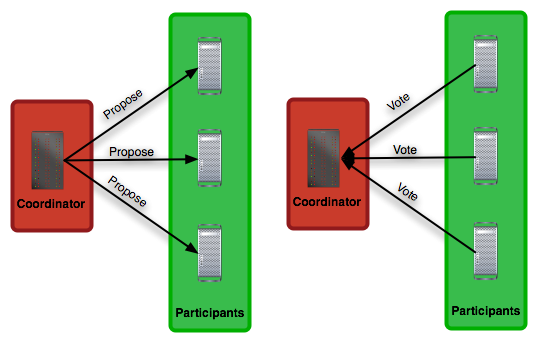
\includegraphics[height=50mm]{images/tpc-fault-free-phase-1.png}\hspace{10mm}
	}
	\subfloat[Phase 2]
	{
	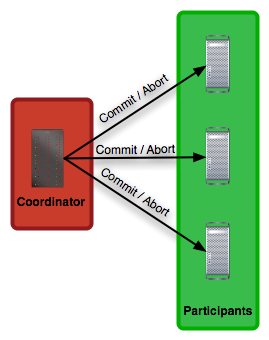
\includegraphics[height=50mm]{images/tpc-fault-free-phase-2.png}\hspace{10mm}
	}
	%\label{fig:replicationRing}
	\caption{2 phase commit}
	\label{fig:2phaseCommit}
\end{figure}


\subsection{Distributed transactions}

% TODO rozrysować co czym jest, Raft, Paxos -> distributed consensous algorithm
% RAMP atomic commit

This section presents more algorithms: \emph{3PC}, \paxos, and \emph{Raft} to solve the consensus problem, which can lead to the implementation of distributed transactions. \lwt is the implementation of the distributed transaction, which uses \paxos to provide distributed consensus. \emph{RAMP} is an algorithm, which provides atomic commit.


\subsubsection{3 phase commit}\label{sec:theory:transactions:3pc}
3PC \cite{3phaseC}, depicted on Figure \ref{fig:3phaseCommit}, divides phase 2 of 2PC into two sub-phases: prepare to commit phase and commit phase, thus it has three phases in total. Upon the prepare to commit message nodes enter the state, in which they are able to commit the value, but also to abort and undo any changes made. The key principle behind this phase is to eliminate the possibility that any node actually commits the value before other nodes are aware of the decision to commit.

In case of the coordinator failure, a recovery node takes over the protocol and queries the state of the remaining nodes. If a node that has committed the transaction failed along with the coordinator, then it is known that all nodes received prepare to commit message therefore the recovery node is able to finish the protocol by committing the value. If a node replies that it hasn't seen a prepare to commit message, then it means that none of the nodes received commit yet, thus the recovery node can re-run the protocol. 

\begin{figure}[H]
	\centering
	\begin{tabular}{c}
	\subfloat[Phase 1 propose]
	{
	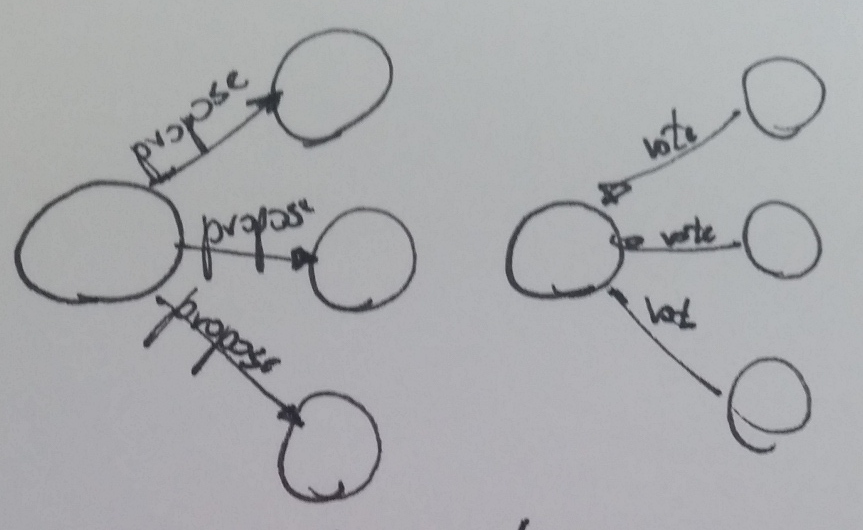
\includegraphics[height=50mm]{images/3pc-phase1.png}\hspace{10mm}
	} \\
	\subfloat[Phase 2 prepare to commit]
	{
	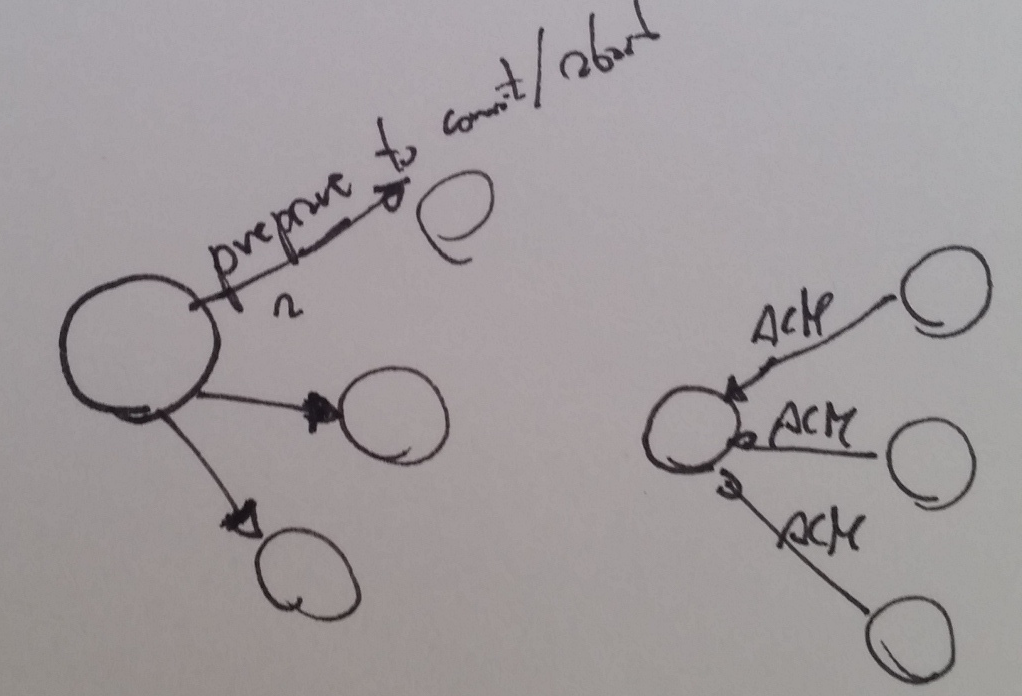
\includegraphics[height=50mm]{images/3pc-phase2.png}\hspace{10mm}
	} \\
	\subfloat[Phase 3 commit]{
		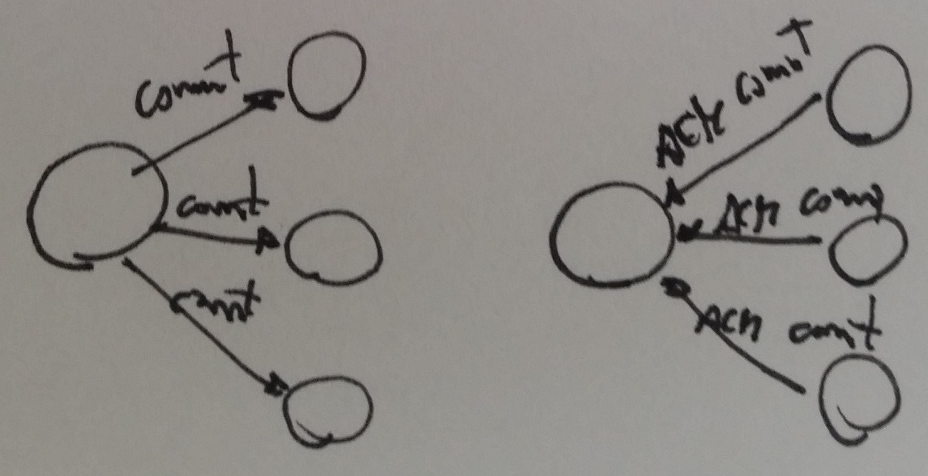
\includegraphics[height=50mm]{images/3pc-phase3.png}\hspace{10mm}
	}
	\end{tabular}
	
	%\label{fig:replicationRing}
	\caption{3 phase commit}
	\label{fig:3phaseCommit}
\end{figure}

\subsubsection{Paxos}
Paxos is another algorithm to solve distributed consensus problem, originally presented in \cite{Lamport1998partTimeParliment}, caused confusion among researchers, due to its complicated explaination and mathematical proofs, and had to be explained in simpler terms in \cite{lamport2001paxosMadeSimple}. 

Paxos was used, as the solution to the distributed consensus problem, as part of the larger systems in \cite{chandra2007PaxosMadeLive}, \cite{lampson1996build}, and more recently in the Google's Chubby service \cite{burrows2006chubby}, which is a lock service intended to provide coarse-grained locking, as well as reliable storage. 

Paxos defines requirements and constraints that the protocol must operate within \cite{lamport2001paxosMadeSimple}. Some of them are: \begin{enumerate}
  \item every proposal has a sequence number called ballot \ballot, that can be generated by any proposer,
  \item majority has to promise to a proposer, before proposer can make proposal,
  \item acceptors reply with a value associated with the highest \ballot already accepted by them. Then proposer is bound to ask acceptors to only commit that value (which might be different from its original proposal) -- this forces proposer to commit other completed proposals instead of his own,\label{sec:mpp:requirements:finishInProgress}
  \item proposer can finish protocol only when majority of acceptors acknowledge commit.
\end{enumerate}

Figure \ref{fig:paxosBasic} shows complete paxos round and exchanged messages between coordinator and nodes. The coordinator \coordinator has to propose new value \paxosValue, therefore it begins next \paxos round represented by a higher ballot \ballot. Nodes which learn new value are called \emph{acceptors}, which arrive at consensus about value \paxosValue after $3$ phases:
\begin{enumerate*}[label=(\alph*)]
\item prepare phase,
\item propose phase,
\item commit phase.
\end{enumerate*}
In prepare phase \coordinator has to establish leadership between acceptors, therefore it sends prepare message with \ballot to nodes \node{1}, \node{2}, \node{3}. An acceptor promises to listen iff \ballot is higher than currently promised. Acceptors responds with the promise and also attaches already accepted proposal. In this case there are no other ballots, nor proposals, thus all nodes promise and \coordinator gains leadership, which allows \coordinator to send proposal.

In propose phase \coordinator sends a message including \ballot and the proposal, which is either one of already accepted proposals received from acceptors or \paxosValue if there are no other proposals pending.
Acceptors check if their ballot is smaller than the one in the message and if it is then they reply with acceptance. If \coordinator received majority of acceptances then it can commit. If it received majority of rejections then it has to abandon the proposal and start again.

In commit phase \coordinator broadcasts the commit message and waits for majority of acknowledges. If acknowledges do not arrive it has to start over.

\paxos depends only on majorities within each phase, thus is resilient to node failures, therefore \paxos has advantage over \emph{3PC}.

\begin{figure}[H]
  \centering

  \begin{sequencediagram} 
  	\newthread[blue]{c}{:Coordinator node} 
  	\newinst{n1}{:Node 1}
  	\newinst{n2}{:Node 2}
  	\newinst{n3}{:Node 3}

	\mess[1]{c}{prepare ballot}{n1}
	\prelevel
	\mess[2]{c}{prepare ballot}{n2}
	\prelevel
	\prelevel	
	\mess[2]{c}{prepare ballot}{n3}
	
	\mess[1]{n1}{promise}{c}
	\prelevel
	\mess[1]{n2}{promise}{c}
	\prelevel
	\mess[1]{n3}{promise}{c}


	\mess[1]{c}{propose ballot, value}{n1}
	\prelevel
	\mess[2]{c}{propose ballot, value}{n2}
	\prelevel
	\prelevel
	\mess[2]{c}{propose ballot, value}{n3}

	\mess[1]{n1}{accept}{c}
	\prelevel
	\mess[1]{n2}{accept}{c}
	\prelevel
	\mess[1]{n3}{accept}{c}

	\mess[1]{c}{commit ballot}{n1}
	\prelevel
	\mess[2]{c}{commit ballot}{n2}
	\prelevel
	\prelevel
	\mess[2]{c}{commit ballot}{n3}
	
	\mess[1]{n1}{ack}{c}
	\prelevel
	\mess[1]{n2}{ack}{c}
	\prelevel
	\mess[1]{n3}{ack}{c}
\end{sequencediagram}

	
  \caption{Paxos failure-free round}
  \label{fig:paxosBasic}
\end{figure}


% These are requirements that need to be satisfied in order to be sure that \paxos can work the way it was designed and proven formally \cite{Lamport1998partTimeParliment}. 

%\paragraph{Paxos guarantees}
%\label{sec:theory:paxos:guarantees}
%TODO co gwarantuje Paxos, tak zeby opis Rafta do tego nawiazywal ale bez referencji, bo Raft jest zaraz po Paxosie.

% \begin{example}

% 	TODO przyklad Paxosa, jakos trzeba go wytlumaczyc

% \end{example}

% TODO opisać na tyle szczegółowo żeby móc je porównać. 
% bez dokładnego schematu
% ogólny schemat, najbardziej typowy przypadek opisać, bez dowodów, bez wyników testów.
% żeby było wiadomo o co chodzi.

% po to żeby móc porównać, Paxos jest lepszy od 3PC bo (ma partycje) i źródło "dokładnie jest to opisane tu i tam"
% ma wynikać z jakiego powodu jest lepszy


%  Paxos, Raft, 3PC opisane na jednym poziomie szczegółowości

% żeby do zrozumienia pracy nie trzeba było zaglądać gdzieś indziej.


\subsubsection{Raft}
% TODO napisać jakie to są guarantees
%\emph{Raft} algorithm offers the same guarantees, as \paxos. 
The aim of \emph{Raft} designers was to create a consensus algorithm which would be more understandable to its predecessor \cite{ongaro2014search}. 
The main idea behind the algorithm is decomposition of the consensus problem into the following individual tasks:
\begin{enumerate*}
\item leader election,
\item log replication,
\item safety,
\item membership changes.
\end{enumerate*} 
%Safety property is that: if any server
%has applied a particular log entry to its state machine,
%then no other server may apply a different command for the same log index.
 
 A server supporting \emph{Raft} is in one of three states: \begin{enumerate*} \item leader, \item follower, \item candidate \end{enumerate*}. The leader can be only one and it handles all client requests.
  When a follower, which is a node listening to the leader, does not receive an heartbeat message within specific time it becomes the candidate and requests election votes from other nodes. If it receives the majority of votes it becomes the leader for the next \emph{term}. Client's request is handled by the leader, which saves the value in uncommitted state in its log and communicates the value to the followers, which acknowledge it. Upon majority of acknowledges the value is committed at the leader node, and the followers are notified about the commit on the next heartbeat message. The leader responds to the client, as soon as the value is committed just at the leader node. When a follower, receives a request from a client, it has to redirect request to the leader.

  \emph{Raft} is resilient to network partitions, since the candidate has to acquire majority of the votes. If there is a split vote, which means that two nodes are candidates which received same number of votes, the election begins again in the next term after a timeout, thus there is only one leader.
  \emph{Raft} algorithm is visualized in \cite{raftVisual}.

% TODO reszta opisu

 %The difference to \paxos  is that \emph{Raft} has been decomposed into independent subproblems which clearly address problems. 

% TODO %
% Napisać jak ten RAFT działa
%\emph{Raft} uses \emph{Leader election}. Leader is elected for specific term. \emph{Raft} uses \emph{Log Replication} to arrive at consensus. Leader proposes new value to \emph{followers} which append value to uncommitted log. Once leader has majority of acknowledges it sends commit message. Followers receive commit message and commit value in the log. 



\subsubsection{RAMP}\label{sec:theory:transactions:ramp}
\emph{Read Atomic Multi Partition} transactions \cite{Bailis:2014} is the newest algorithm among the algorithms discussed in this chapter. 
\emph{RAMP} algorithm was designed to address the requirements of the following use cases: secondary indexing, foreign key
enforcement, and materialized view maintenance.
\emph{RAMP} identifies new transaction isolation level \emph{Read Atomic}, which 
assures consistent visibility of changes made by the transaction: either all or none of each transaction's updates are seen by other transactions.
\emph{RAMP} is resilient to failures of part of the nodes in the cluster -- for the reason that RAMP's transaction does not contact nodes that are not affected by the transaction. 
\emph{RAMP} also guarantees \emph{synchronization independence}, which means that transactions do not stall or fail other transactions, due to the fact that reads and writes do not block each other. 

%The transaction is able to detect non-atomic partial read and repair it with additional rounds of communication with nodes. 
The key principle behind \emph{RAMP} is its ability to detect non-atomic partial read, and to repair it with additional rounds of communication with the nodes by the means of \emph{the metadata} attached to each write and \emph{multi-versioning}, which means that the data is accessible in different versions and each modification to the data creates a new version. Versions are either committed or not yet committed, in which case the data can be discarded by aborting the transaction \cite[p. 6]{Bailis:2014}. 
There are three variants of \emph{RAMP} algorithm which differ in type of the metadata. \emph{RAMP-small} uses a 64 bit timestamp as the metadata and requires additional two rounds of communication when non-atomic read is detected. Other variants of \emph{RAMP} are described in \cite[p. 5]{Bailis:2014}.
\emph{RAMP} is linearly scalable, which was tested during trials with the number of nodes spanning up to 100 servers \cite[p. 10]{Bailis:2014}.

%  TODO Może to gdzieś się opłaca dodać:
% \emph{RAMP} transactions \ref{sec:theory:transactions:ramp} have support for multi-partition operations. 
% However \emph{RAMP} relies on 64 bit timestamp \cite[p. 8]{Bailis:2014} which is not the current standard \cite{timestamp64wiki}, thus \emph{RAMP} cannot be used at the time being.
%

\subsubsection{LWT}\label{sec:theory:transactions:lwt}
% TODO źródło w (more on this)
As mentioned earlier, Light Weight Transactions is the name of compare-and-swap functionality implemented in Cassandra. Internally, LWT uses the Paxos algorithm with some modifications which were aimed to prevent potential single point of failure, thus improving high availability. SPOFs may surface in case the leader fails when it is about to propose a new value. The problem was addressed by sacrificing the standard leader election in favour of allowing any node to act as a leader, so that it can propose a value at any time. On the downside, such approach increases the risk of contention. 

One of the key requirements of Paxos protocol is storage of PaxosState - a data structure composed of the proposed value, proposed ballot, promised ballot and most recent commit. In case of LWT, the value represents the update itself along with the token of the partition key where that update should be applied. That token uniquely identifies PaxosState so that several proposals for the same partition can be associated with the same Paxos instance. 


LWT includes the following phases: \begin{enumerate*}
\item prepare,
\item get promise,
\item read row,
\item get results,
\item propose a new value,
\item acceptance,
\item broadcast commit,
\item wait for acknowledgements.
\end{enumerate*} 

Let us analyze each of them in the environment with \N{5}, \RF{3} and request to insert user named \emph{John} to \emph{users} table, but only if \emph{John} does not exist. For simplicity, \emph{users} table has only two columns: \begin{enumerate*} 
\item name -- text column and primary key, \item email -- text column. \end{enumerate*} \lwt begins with a node 5 receiving request. Node 5 is then called coordinator node. The coordinator has to become the leader of paxos round identified by the token computed from partition key of \emph{users} table, thus from string value \emph{John}. To become the leader, the coordinator has to create the new ballot and send it along with the token and table name to replica nodes: node 1, node 2, node 3. Each replica has to check whether the ballot is the highest ballot it has seen, and if it is, then replica saves it in the PaxosState and responds with a promise. The leader has to wait for majority of promises before it proceeds. When majority promises, the coordinator may proceed to read the row and check the condition. The condition is that \emph{John} cannot exist, thus read has to not find any rows querying users by user name \emph{John}. Let us assume that indeed user \emph{John} did not exist, thus condition is met which allows the coordinator to propose an insert of \emph{John} with email \emph{john.doe@gmail.com} to \emph{users} table. The coordinator sends proposal message, with an insert and same ballot, to replicas and waits for acceptances. A replica saves proposed insert to PaxosState and replies with acceptance message.
When the coordinator receives majority of acceptances it broadcasts the commit message and waits for majority of acknowledgements. Upon receiving commit message a replica applies an update stored in PaxosState, thus it performs the insert of \emph{John} to \emph{users} table and acknowledges commit with a reply.

At any time during whole procedure the minority of replicas might stop responding and LWT can continue. In case of the example, one node can fail without aborting \emph{LWT}. If more than one node fails, then LWT is aborted. 

Secondly, at any time the leader might lose leadership if other node does prepare with a higher ballot. In that case the coordinator has to wait, giving the other leader time to complete its \lwt, and try again with new ballot.

Note that \lwt affects only limited number of nodes -- replicas of \emph{John}, thus majority is considered only at the level of replicas, not at the level of the cluster.

\lwt is limited to a single partition, thus \lwt cannot be used for atomic updates of many partitions, thereby this paper presents a new algorithm, which overcomes limitations of \lwt.
The proposed algorithm supports multi-partition operations, and provides read-committed isolation level, whereas \lwt provides serializable isolation.

%1. LWT is initiated by client request: insert John if not exists
%2. Request is routed to some node X that becomes coordinator of LWT
%3. Coordinator wants to be a leader so it creates a ballot and sends prepare to replicas: node1, node2, node3. This is prepare phase.
%4. Replicas promise to not accept values from leaders who have lower ballots.
%5. Coordinator gets 3 of out 3 promises. Quorum promised to listen.
%6. Coordinator performs read: SELECT * FROM users WHERE user_id = 1
%7. Coordinator checks condition “IF NOT EXISTS”. If such row did not exist in quorum of replicas it proceeds further
%8. Coordinator, as a leader, proposes new value which is an insert to users table.
%9. All three nodes reply with accept. Quorum accepted insert.
%10. At this point, insert is an in progress proposal that has been accepted by majority of replicas. Even if coordinator crashes, once someone selects user with id=1 or retries to insert it. This proposal will get committed. Let’s assume that coordinator is well and proceeds to commit.
%11. Coordinator broadcasts commit message
%12. Replicas apply insert locally and reply with acknowledge message
%13. Coordinator receives quorum of acknowledges. LWT has been successfully completed.
%14. Coordinator responds to client: John was inserted.


%Sequence above is a happy path. At any point coordinator might lose his leadership if some other node sends prepare with higher ballot. In that case coordinator waits a bit and retries whole process again. 
%Also any replica might stop responding, which is fine as long as quorum is up and well. If quorum responds to messages, coordinator can proceed. If there is no quorum then paxos conditions are not met and LWT cannot be continue. However during normal operation is it rather rare to see many nodes down so in general LWT can successfully finish with 2 out of 3 replicas running. Note that cluster size might be much bigger, for example hundred nodes, but since replication factor \RF{3}, only three nodes are interesting from perspective of LWT and Paxos.
